\section{Gobernanza}
  \label{Solucion:Gobernanza}

  \subsection{Modelo de jurisdicción}
    \label{Solucion:Gobernanza:ModeloJurisdiccion}
    De las conclusiones del análisis de la realidad se desprende la capacidad limitada de AGESIC para influir en el análisis y definición de inventarios de servicios, dado que las etapas iniciales suceden en los organismos en forma independiente. Considerar una opción agresiva en la cual los organismos debieran consultar con AGESIC constantemente durante el diseño de servicios, podría afectar negativamente al proceso de creación de los mismos en cada organismo por separado, y esto además, sin tener en cuenta la capacidad de esfuerzo con la que cuenta la agencia al momento de aplicar este protocolo. Por otro lado, dado que la información manipulada por cada organismo es propiedad exclusiva de estos, y cualquier intercambio de información ocurrirá con previa autorización legal, se puede asumir que ningún organismo publicará información de otro a través de sus servicios. Esto es interpretable como un indicador de \emph{bajo riesgo de superposición de servicios} entre organismos, una de las dos motivaciones para la separación en inventarios. Con este aspecto en mente, es posible delinear dominios que abarquen a los servicios de un mismo organismo proveedor, dejando así en manos de estos el diseño de servicios re-utilizables y con responsabilidades separadas dentro de su propio inventario.

    En concordancia con la idea de centralizar los servicios dentro de una misma plataforma, es necesario establecer determinados criterios con los que los servicios deben cumplir, separados de las recomendaciones sobre el diseño que se crean pertinentes. AGESIC debe establecer procesos estandarizados para la publicación de nuevos servicios en la PDI, a través de los cuales se verificará la compatibilidad de los servicios con los requerimientos establecidos —tal y como sucede en la plataforma actual, en donde los organismos trabajan en el diseño e implementación de sus servicios y luego realizan la solicitud a AGESIC para publicarlos en la PDI, por lo que gran parte de la gobernanza sobre el diseño e implementación, ocurre en forma independiente dentro del organismo.

    Tomando estas consideraciones en cuenta es que se propone una variante del modelo de jurisdicción de SGPO por dominio federado, cumpliendo así con la agrupación de servicios por organismo, manteniendo la independencia en la gobernanza por parte de cada uno y a su vez estableciendo una SGPO central (AGESIC) encargada de establecer las políticas comunes a todos los organismos para el diseño de sus servicios conforme a los requerimientos de la PDI. La variante del modelo se da en los casos en que el organismo en cuestión cuenta con una estructura de gobernanza más compleja que una única SGPO centralizada para todos sus servicios. Esto último ocurre en casos en que más de un dominio es gobernado por el organismo; bajo esta situación, no se puede realizar una adaptación exacta a los modelos de jurisdicción presentados en el framework de base, ya que el organismo podría implementar su propio modelo de jurisdicción tomando como referencia su SGPO central, generando así más niveles de SGPO que los identificados en los modelos vistos.

    En la figura \ref{imagen:modelo_jurisdiccion_sgpo_propuesta} se muestra el modelo de jurisdicción de la propuesta. Una línea punteada horizontal entre las SGPO de los organismos y los inventarios representa la posibilidad de los primeros de implementar su propio modelo de jurisdicción. Si bien la cantidad de dominios o inventarios puede diferir a la vista del organismo, desde la perspectiva de AGESIC, siempre se tomará el conjunto de servicios publicado por un organismo como parte de un único dominio.

    \begin{figure}
      \centering
      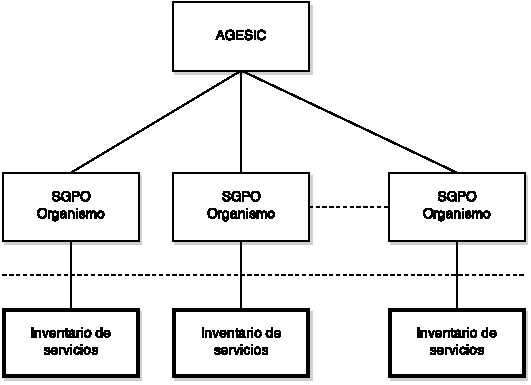
\includegraphics[width=\linewidth]{modelo_jurisdiccion_sgpo_propuesta}
      \caption{Modelo de jurisdicción de SGPO propuesto}
      \label{imagen:modelo_jurisdiccion_sgpo_propuesta}
    \end{figure}

  \subsection{Ciclo de vida de servicios}
    \label{Solucion:Gobernanza:CicloDeVida}
    Los organismos tienen independencia no sólo en el sistema de gobernanza que aplican a sus servicios, sino también en el que aplican a su infraestructura de publicación, mientras que AGESIC tiene jurisdicción sobre la infraestructura intermediaria entre los consumidores y la de los organismos proveedores, es decir, sobre la PDI. Esto hace necesario divergir del proceso en etapas básico del framework, visto en la sección \ref{MarcoConceptual:GobernanzaSOA}, y agregar etapas que cubran la negociación para la publicación de los servicios alojados en la infraestructura del organismo, en la PDI.

    \begin{figure}[h]
      \centering
      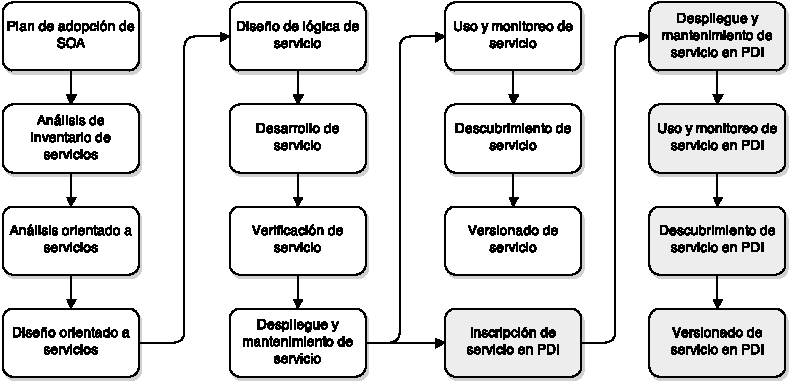
\includegraphics[width=\linewidth]{ciclo_de_vida_propuesta}
      \caption{Ciclo de vida de proyecto y servicios propuesto}
      \label{imagen:ciclo_de_vida_propuesta}
    \end{figure}

    En la figura \ref{imagen:ciclo_de_vida_propuesta} se presenta la secuencia propuesta para la publicación, monitoreo y versionado de servicios en la PDI gobernada por AGESIC, desde el inicio de su concepción en los organismos, pasando por su publicación en la infraestructura propia hasta llegar al subproceso de publicación en la plataforma. Las etapas contrastadas son las gobernadas por AGESIC y comienzan a partir de la solicitud de publicación de un servicio. Las etapas anteriores a la solicitud de publicación de la figura \ref{imagen:ciclo_de_vida_propuesta} funcionan a modo de ejemplo basado en las etapas de un proyecto SOA vistas en la sección \ref{MarcoConceptual:GobernanzaSOA}. La gobernanza en SOA de cada organismo permanece independiente y por lo tanto, no se establece que esas deban ser las etapas que los mismos deban seguir, aunque se recomienda la adopción de la gobernanza en SOA como herramienta central en la gestión de cada arquitectura.

  \subsection{Gobernanza del ciclo de vida en AGESIC}
    \label{Solucion:Gobernanza:CicloDeVidaAGESIC}

    Ante la necesidad de proveer un nuevo servicio a través de la PDI, el organismo deberá contactar con AGESIC para hacer que el servicio se encuentre dentro de la plataforma y sea accesible por otros organismos. El proceso se describe en la figura \ref{imagen:proceso_publicacion_pdi}.

    \begin{figure}[h]
      \centering
      % Pendiente
      \caption{Diagrama BPMN del proceso de publicación en la PDI}
      \label{imagen:proceso_publicacion_pdi}
    \end{figure}

    \begin{enumerate}
      \item Inscripción de servicio
      \item Despliegue y mantenimiento de servicio
      \item Uso y monitoreo de servicio
      \item Descubrimiento de servicio
      \item Versionado de servicio
    \end{enumerate}

    \subsection{Inscripción de servicio}
      \label{Solucion:Gobernanza:CicloDeVidaAGESIC:Inscripcion}
      % Se había comentado de un sistema de formulario vía web en lugar de continuar con la utilización de papel como se hace hoy en día.
      \emph{Próximamente}
      \emph{Se maneja la idea de crear un formulario web para la gestión del proceso, en lugar de lo que se hace hoy en día mediante papeleo. Acá se debería hablar sobre inscripción, generación de SLAs entre AGESIC y el proveedor, etc.}

    \subsubsection{Despliegue y mantenimiento}
      \label{Solucion:Gobernanza:CicloDeVidaAGESIC:Despliegue}

      En esta etapa se lleva a cabo la configuración del acceso al servicio por parte de los consumidores a través de la PDI. Se asume completada la etapa de implantación en la plataforma del proveedor. En este caso, el objetivo es configurar una comunicación entre la PDI y el servicio desplegado del lado del organismo, de modo que los clientes de dicho servicio establezcan la comunicación con el lado del proveedor a través de la PDI de forma transparente. Para lograr esta comunicación se utilizará una tecnología que permita crear ``proxies" en la PDI, preconfigurados para redirigir el tráfico hacia la infraestructura del proveedor como se muestra en la figura \ref{imagen:cliente_pdi_proveedor}. Ejemplos de este tipo de tecnología son los \emph{Enterprise Service Bus (ESB)} de proveedores conocidos como JBoss\footnote{https://www.jboss.org/jbossesb/} o IBM\footnote{\url{http://www.ibm.com/software/products/en/wsesb/}}. Los procedimientos en cuanto a configuraciones de seguridad y acceso están fuera del alcance de esta propuesta. Se sugiere mantener las características actuales.

      \begin{figure}[h]
        \centering
        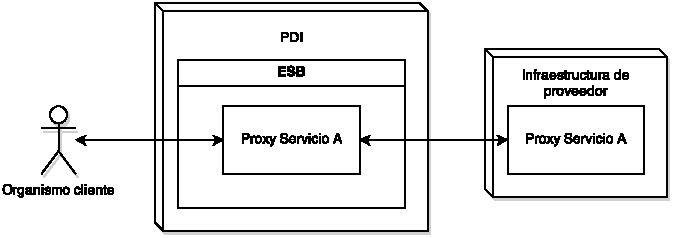
\includegraphics[width=\linewidth]{cliente_pdi_proveedor}
        \caption{Patrón «Proxy» aplicado a la comunicación entre cliente y proveedor}
        \label{imagen:cliente_pdi_proveedor}
      \end{figure}

      El rol de \emph{desarrollador} participa en las actividades llevadas a cabo en esta etapa, recibiendo la especificación del servicio para realizar las configuraciones pertinentes en la infraestructura de software de la PDI. Dicha especificación es obtenida a partir del proceso descrito en la sección \ref{Solucion:Gobernanza:CicloDeVidaAGESIC:Inscripcion}.

      Al completarse el proceso de configuración, se entra en fase de verificación para asegurar el cumplimiento de los requisitos de funcionamiento del servicio, así como también de los de calidad establecidos en el acuerdo de nivel de servicio (siglas en Inglés, SLA) entre AGESIC y el proveedor. El rol de \emph{especialista en el aseguramiento de la calidad (QA, por sus siglas en inglés)} dirige los procesos de verificación llevados a cabo, es decir, todos aquellos que aseguren una correcta comunicación entre la infraestructura de la plataforma de interoperabilidad y la del organismo proveedor del servicio, así como también el correcto funcionamiento de los controles de seguridad y acceso. No se verifica el funcionamiento en cuanto a la lógica del servicio en cuestión sino únicamente una comunicación exitosa; este tipo de verificación se asumirá completada por parte del organismo proveedor al momento de realizar el despliegue.

      El mantenimiento es un trabajo conjunto entre desarrolladores y especialistas en QA. Este implica una verificación periódica de los sistemas que mantienen al servicio disponible a través de la PDI y especialmente, en cumplimiento con su SLA a través de las métricas establecidas en el modelo de calidad aplicado. AGESIC debe encargarse de las tareas de mantenimiento necesarias para mantener la comunicación entre la PDI y el servicio del ldo del proveedor funcionando como se espera. Estas tareas de mantenimiento pueden requerir en ocasiones, una baja temporaria del servicio, afectando así a la disponibilidad. Se debe tomar en cuenta para evitar mayores dificultades, los horarios de uso establecido por los consumidores para realizar dichas tareas fuera de los horarios «pico» de utilización. Independientemente de la franja horaria en la que se realicen las tareas de mantenimiento, se deberá dar notificación de aquellas que sean programadas, en forma electrónica e inmediatamente luego de ser agendadas. Se proponen dos vías simultáneas como base: un servicio de novedades de tipo «feed de noticias» o alimentador, y comunicación vía correo electrónico a las direcciones de contacto provistas por los clientes. Esto permite a cualquier usuario del sistema, acceder a información sobre el estado de mantenimiento de los servicios, y permite la notificación en caso de que no exista una conducta de verificación regular del estado.

      Una tercera vía a implementar puede ser tomada de \emph{Google Apps Status Dashboard}\footnote{\url{http://www.google.com/appsstatus}}. Esta consiste en un sistema que lista los servicios disponibles y establece un color para el estado reportado en el que se encuentran al momento de ingresar al sitio. Cuando suceden errores que son detectados, u ocurren tareas de mantenimiento programadas, estas son identificadas con el color apropiado en dicho sitio.

      \emph{En desarrollo}

    \subsubsection{Uso y monitoreo}
      Durante el uso y monitoreo de los servicios, AGESIC se encargará de recolectar los valores de las mediciones correspondientes para asegurar la calidad y buen funcionamiento del servicio, así como también servir de retroalimentación para las actividades de mantenimiento y cobro por acceso.

      Periódicamente se realizarán actividades de revisión de funcionamiento sobre los servicios para determinar la necesidad de realizar ajustes sobre la configuración del acceso, independientemente de las revisiones de vitalidad que se realicen bajo la gobernanza del propio organismo sobre la lógica del servicio.

      Para realizar estas revisiones se tomarán en cuenta atributos de calidad que tengan impacto sobre la carga del servicio. Por ejemplo, un servicio que esté experimentando «picos» de uso periódicamente, deberá someter su configuración a revisión por parte del equipo de analistas de AGESIC para determinar la necesidad y viabilidad de un aumento de recursos para el proxy intermediario.

      Para hacer posible la detección de estas situaciones, se contará con un sistema de monitoreo sobre los servicios, el cual estará configurado en base a un modelo de calidad (abordado en la sección \ref{Solucion:Calidad}). No se especifica en esta propuesta una forma de monitoreo particular; en base a la infraestructura existente, se sugiere la instalación de módulos de medición de atributos de calidad en la infraestructura de un Enterprise Service Bus (ESB).

      \emph{En desarrollo}

    \subsubsection{Descubrimiento}
      Siguiendo el principio de \emph{Service Discoverability} (una ponderación sobre qué tan sencillo es encontrar un servicio), será necesario hacer que los servicios dispongan de suficientes meta-datos que permitan a un potencial usuario, descubrirlo y reutilizarlo en sus procesos de negocio, de manera de no solicitar la creación de nuevos servicios que cubran en todo o en parte lo que servicios ya existentes.

      Para facilitar el descubrimiento se establece una serie de meta-datos básicos de los que todos los servicios deben disponer. Esta información será desplegada en un registro central (central registry), gobernado por AGESIC. Este registro será independiente de los posibles registros gobernados por cada organismo, ya que contendrá sus propios meta-datos predefinidos y almacenados al momento de la publicación/migración.

      El acceso a este registro será público a través de la Internet. El sitio web se hará disponible a través de un servidor web gestionado por AGESIC. Se aplicará un criterio de confidencialidad sobre los meta-datos “sensibles”, de forma de no hacerlos disponibles a través del catálogo público, de existir.
      Algunos servicios podrán requerir ser marcados como privados, y por tanto sólo descubribles a en forma interna y con acceso autorizado. Esto deberá someterse a evaluación por parte del proveedor del servicio, en caso de que así se indique en la solicitud de publicación.

      Personal en el rol de custodio de servicios se encargaran de revisar los datos de los servicios publicados para asegurar la completitud y veracidad de los mismos. Un mismo custodio podrá estar encargado de más de un inventario de servicios, de ser necesario; no se establecen restricciones al respecto.

      El registro no permitirá la gestión del acceso al servicio a través de la web, sino que se continuará con el procedimiento actual de gestión de la publicación a través de formularios. Se sugiere con énfasis la implementación de un sistema electrónico independiente para la gestión de la publicación y solicitud de implementación de servicios.

      Ante situaciones de descubrimiento de servicios que resulten en solicitudes de modificaciones, las mismas serán transmitidas al organismo proveedor responsable y se pondrá en contacto al solicitante con dicho proveedor para negociar los cambios, los cuales, podrían resultar en una posterior migración de versión, situación descrita en la próxima sección.

      Una buena etapa de descubrimiento de servicios, requiere de la participación en la etapa del diseño orientado a servicio. Sin embargo, como hemos visto, AGESIC no participa de dicha etapa, por lo que la definición o modificación de meta-datos de uno o más servicios, puede requerir de contactar a los diseñadores responsables de cada uno.

      En la sección \ref{Implementacion:CasoEstudio} introducimos una descripción de la implementación de un prototipo de registro central de servicios.

      \emph{En desarrollo}

    \subsubsection{Versionado y retiro}
      Una nueva versión de un servicio será gestionada a partir de la solicitud por parte del organismo responsable. El procedimiento para la solicitud será similar al de la publicación, con el rellenado de un formulario especificando información relevante al cambio de versión. Esta actividad puede requerir de interacción entre responsables para determinar el procedimiento a seguir en cuanto a la configuración de la PDI y los cambios que potencialmente será necesario realizar para mantener el funcionamiento.

      Se aplicará la técnica de versionado desarrollada en la sección A DEFINIR.

      El retiro definitivo de servicios deberá ser planificado y anunciado cuanto antes a los organismos dependientes, de forma de permitirles establecer un curso de acción. Esto puede resultar difícil si el organismo proveedor omite el anuncio a AGESIC sobre la pre-determinación del retiro. Lo ideal será considerado que un servicio se encuentre en estado «deprecated» por un periodo no menor a 90 días, y esto sea anunciado con igual anticipación a los organismos dependientes. Pasado el periodo, el servicio (Proxy) será dado de baja de la PDI, así como también las configuraciones de seguridad y control de acceso establecidas para el mismo.

      Para determinar las dependencias, se utilizará un registro de consumidores de cada servicio, disponible desde el momento de cada suscripción.

      \emph{En desarrollo}
